\documentclass{zettel}

%\renewcommand{\gregor}{\put(10.0,-3.5){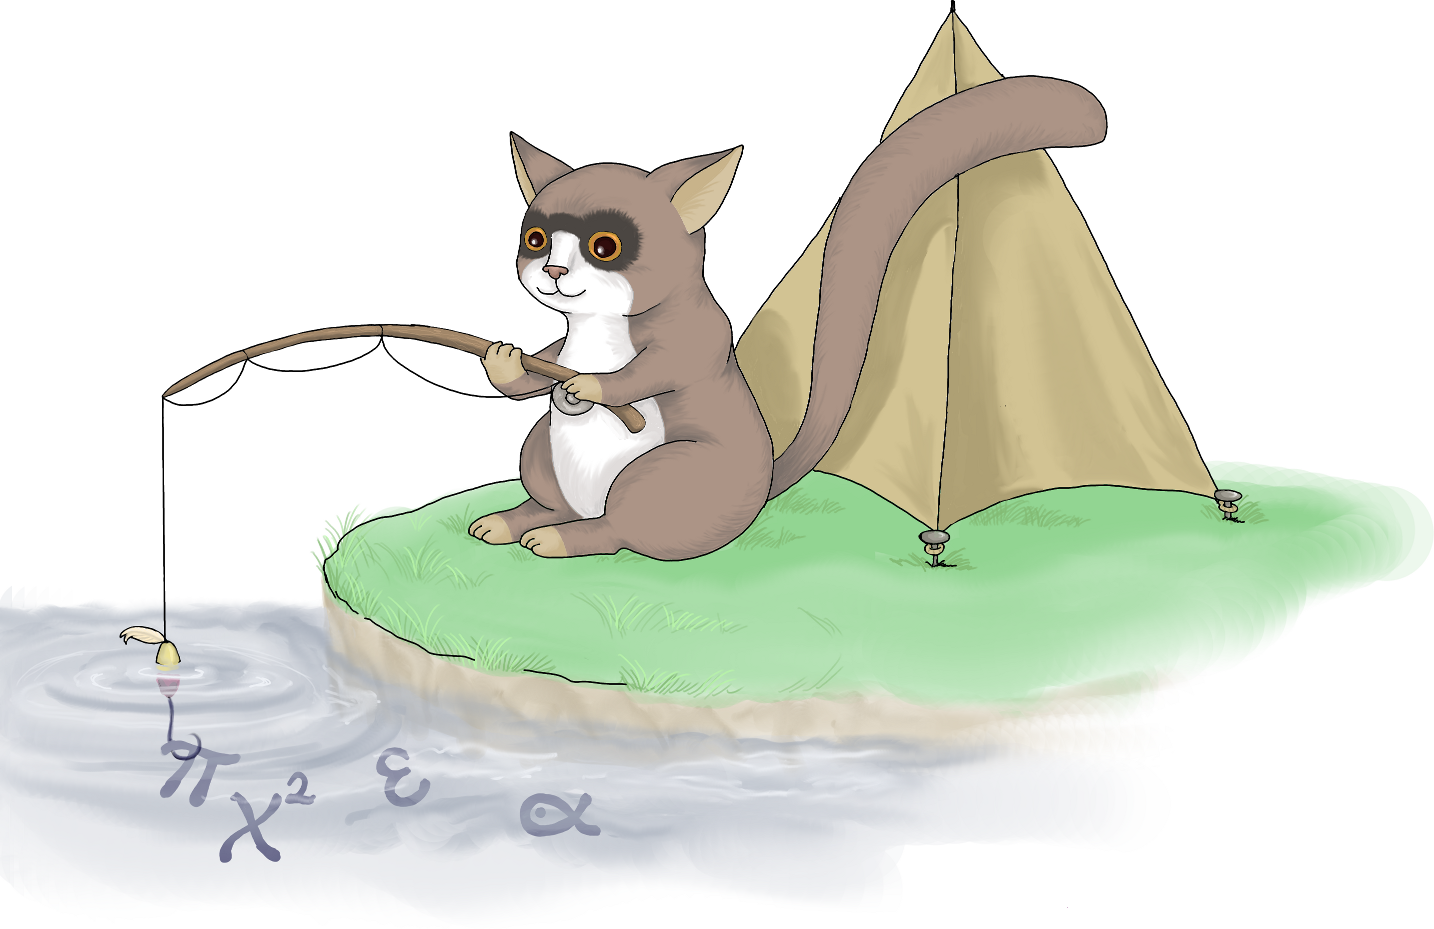
\includegraphics[scale=0.18]{campgregor}}}

\usepackage{framed}
\definecolor{shadecolor}{rgb}{.97,.97,.97}

\geometry{tmargin=1.5cm,bmargin=1.5cm,lmargin=2.5cm,rmargin=2.5cm}

\renewcommand{\gregor}{\put(13.2,-3.0){
\includegraphics[scale=0.18]{cover}}}
\begin{document}

\renewcommand{\betreff}{Mathecamp des Matheschülerzirkels Augsburg vom 16. bis
20. August}

\makeletterhead{}
\begin{picture}(0,0)
  \put(8.4,-19){%
    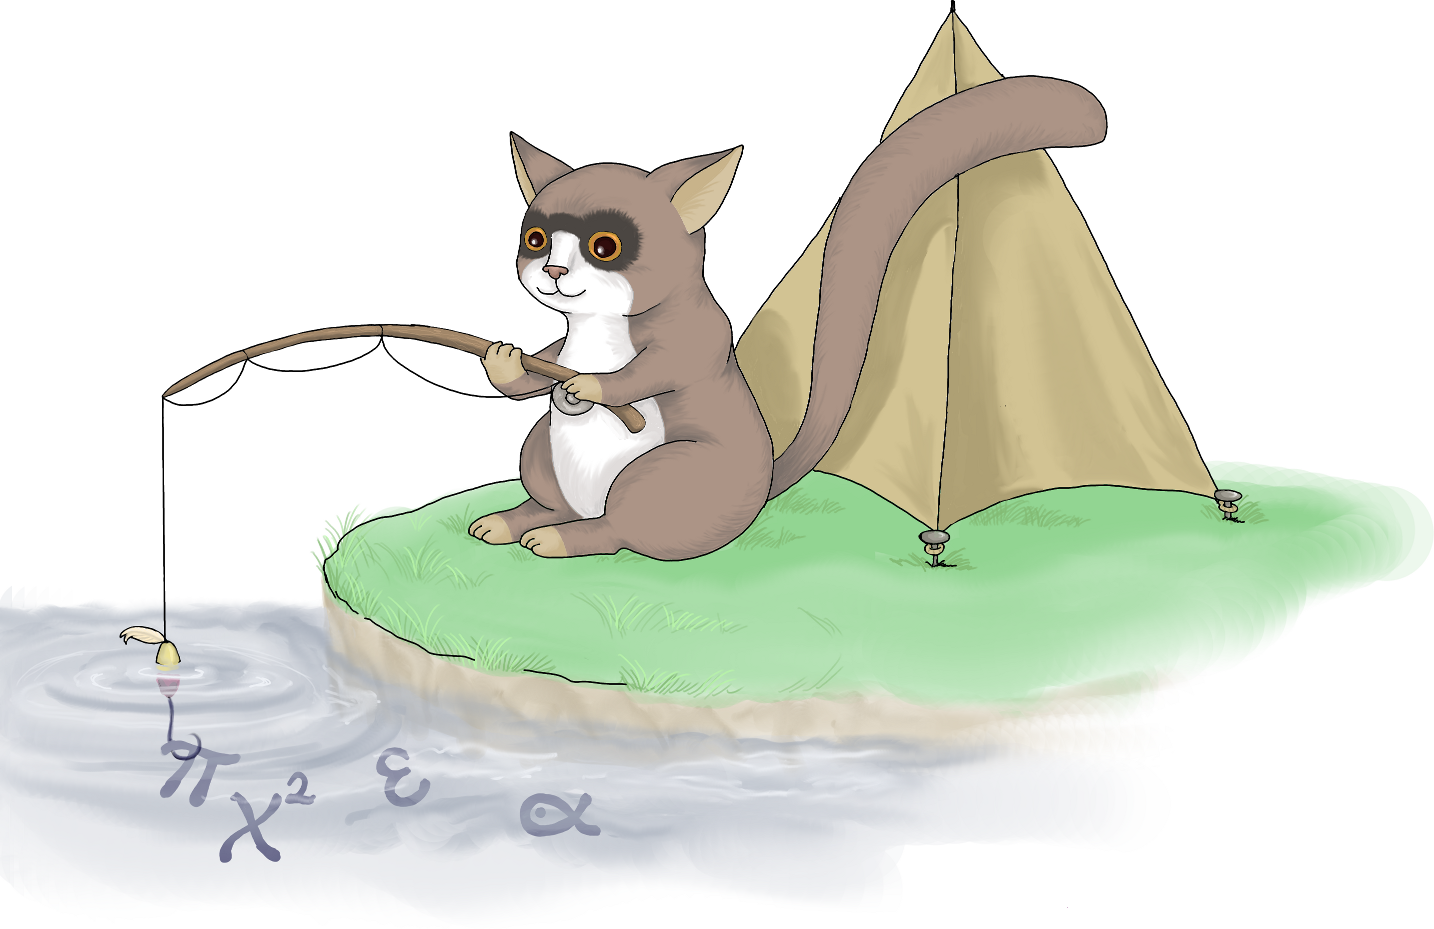
\includegraphics[scale=0.18]{campgregor}
  }
\end{picture}
\vspace{-2em}

Liebe Schülerinnen und Schüler, liebe Eltern,

wir laden euch herzlich zum ersten Mathecamp des Matheschülerzirkels Augsburg
ein. Dort werden wir mit euch tolle mathematische Themen verstehen und die
Freizeit in den Ferien genießen.

\begin{tabbing}
  \hspace{2.2cm} \= \kill
  \textbf{Was?} \> Mathematik und Spaß in den Ferien \\[0.3em]
  \textbf{Wann?} \> 16. bis 20. August 2014 (Samstag bis Mittwoch) \\[0.3em]
  \textbf{Wo?} \> Bruder-Klaus-Heim in Violau (St. Michael Straße 15, 86450
  Violau) \\[0.3em]
  \textbf{Für wen?} \> \begin{minipage}[t]{\dimexpr\textwidth-2.3cm}
  Einzige Teilnahmevoraussetzung ist Spaß und Interesse an
  Mathematik.
  Jeder kann mitkommen, auch, wenn man nicht bei den Zirkeln
  mitgemacht hat.\end{minipage} \\[0.3em]
  \textbf{Kosten?} \> 60,-- \texteuro
\end{tabbing}

An jedem Tag werden zwei Zirkel stattfinden. Dabei behandeln wir spannende
Bereiche der Mathematik, die wir in den Präsenz- und Korrespondenzzirkeln noch nicht gesehen haben.
Selbstverständlich finden die Kurse klassenstufenweise ab. Die restliche Zeit
verbringen wir mit Spielen und Outdoor-Aktivitäten und nutzen das Teleskop und
die Pizzabäckerei unserer Unterkunft. Außerdem wird es zwei Vorträge von
auswärtigen Mathematikern geben.

Getragen wird das Camp vom Mathematisch-Physikalischen Verein e.\,V. Wir
Betreuer sind Doktoranden und Mitarbeiter des mathematischen Instituts.
Wenn ihr teilnehmen möchtet, bittet eure Eltern das beiliegende Anmeldeformular
bis zum 12. Juli 2014 auszufüllen und an uns zurück zu schicken.
\vspace{\medskipamount}

\begin{minipage}{0.54\textwidth}
Dank finanzieller Unterstützung durch das Institut für Mathematik konnten wir
den Eigenbeitrag von ca. 200~\texteuro{} deutlich reduzieren, er beläuft sich
jetzt auf 60~\texteuro. In diesem Betrag sind die Kosten für An- und Abreise,
Unterkunft, Verpflegung und den UnterhaltXXX der Betreuer enthalten.
\end{minipage}

\newpage

Wir bitten, den Betrag bis zum 1. August 2014 auf
unser Konto zu überweisen. Wenn Sie unsere Arbeit zusätzlich unterstützen
möchten, stellen wir Ihnen gerne Spendenquittungen aus. Familien, die sich den
Eigenbeitrag nicht leisten können, bitten wir, mit uns Kontakt aufzunehmen. Im
Rahmen der finanziellen Möglichkeiten unseres Vereins können wir gegebenenfalls
auf den Beitrag verzichten.

\vspace{-0.7em}
\begin{tabbing}
  \qquad\qquad \= Kontoinhaber:\, \= \kill
  \> Kontoinhaber: \> Matheschülerzirkel Augsburg \\
  \> Konto-Nr.: \> 12345678 \\
  \> BLZ: \> 12345678 \\
  \> IBAN: \> 2437243784237878342 \\
  \> BIC: \> 23487432789432
\end{tabbing}
\vspace{-0.7em}

Das Camp beginnt am 16. August zwischen 10:00 Uhr und 11:00 Uhr. Ihr könnt
entweder individuell zu dieser Zeit anreisen oder euch um 09:30 Uhr auf dem Campus der
Universität einfinden, um dann gemeinsam mit uns im Reisebus nach Violau zu fahren.

Die Abreise ist am 20. August ab 16:30 Uhr. Ihr könnt euch entweder von euren
Eltern abholen lassen oder mit uns zurück nach Augsburg fahren. Dort kommen wir
um 17:30 Uhr an der Universität an.

Wir schicken euch in der letzten Juliwoche eine Übersicht mit
letzten Details und Kontaktdaten vor Ort. Bei Fragen stehen wir euch jederzeit
zur Verfügung. Bitte zögert nicht, uns dazu telefonisch unter 0821/598-5805 oder per
Mail an \textsf{mathezirkel@math.uni-augsburg.de} zu kontaktieren.

Wir hoffen, dass ihr euch auf das Mathecamp genauso freut wie wir und dass wir
euch dort begrüßenXXX dürfen!

\vspace{2em}

Euer Team vom Mathecamp

%Übrigens organisieren wir vom 16. bis 20. August ein Mathecamp in Violau. Dort
%bieten wir euch spannende mathematische Kurse und Workshops, etwa zu geheimen
%Botschaften, Fraktalen, Knobelaufgaben, Geometrie, Nim-Spielen oder anderen
%Themen. Daneben gibt es bei unserer Unterkunft auch verschiedene Möglichkeiten
%zur Freizeitgestaltung, unter anderem ein Teleskop, eine Pizzabäckerei und
%Outdoor-Aktivitäten. Wir sind gerade auf Sponsorensuche und werden euch in
%einem Monat nähere Informationen schicken. Wenn ihr Interesse habt, sagt euren
%Eltern schon mal den Termin!

\end{document}

XXX: Euro-Zeichen
